\Introduction

За последние 10 лет большое распространение в промышленности получили манипуляционные роботы, способные решать большой спектр задач, начиная от перемещения объектов и механической обработки деталей, заканчивая сортировкой и дефектоскопией. Исследования в области силомоментного управления в период 70---90-ы гг. прошлого века позволили использовать манипуляционных роботов в задачах, где важно соблюдение технологического процесса с заданными показателями точности к усилию и импульсу, которые сообщаются объектам манипулирования или обрабатываемым деталям. Так появились два класса алгоритмов силомоментного управления: непрямые и прямые \cite{Handbook}. Оба этих метода актуальны и сегодня, каждый из них имеет свои особенности и сферы применения. В данный период многими знаменитыми учеными были изучены, а также сформулированы и описаны методы силомоментного управления \cite{Khatib1986_force_control, Villani2016, Salisbury1980, Yoshikawa1987, RaibertMH;Craig2015}. С 1990 по 2010 в связи с повышением спроса со стороны промышленной индустрии \cite{Yamada1995, Handbook, Yoshikawa1990} на согласованное использование нескольких манипуляторов в общем рабочем пространстве было проведено большое количество исследований алгоритмов кооперативного управления манипуляторами. Актуальность вопроса была также обусловлена необходимостью разработки математического аппарата для унификации синтеза алгоритмов схватывания, энергетически оптимального, а также адаптивного к форме объекта манипулирования \cite{Takahashi2008,Yoshikawa1991, Park1989}.\\

В последнее двадцатилетие появилась высокая потребность в алгоритмах кооперативного управления не только многопалыми схватами, но и промышленными манипуляторами. Тенденции к развитию были сформированы благодаря распространению антропоморфных роботов, имеющих большой потенциал выполнять координационно достаточно сложную работу, подобно человеку. На сегодняшний день антропоморфные роботы стали примером концепции создания роботов, пригодных для функционирования в среде человека, тем самым дав дорогу для развития коллаборативной робототехники.

\begin{figure}[ht]
  \centering
  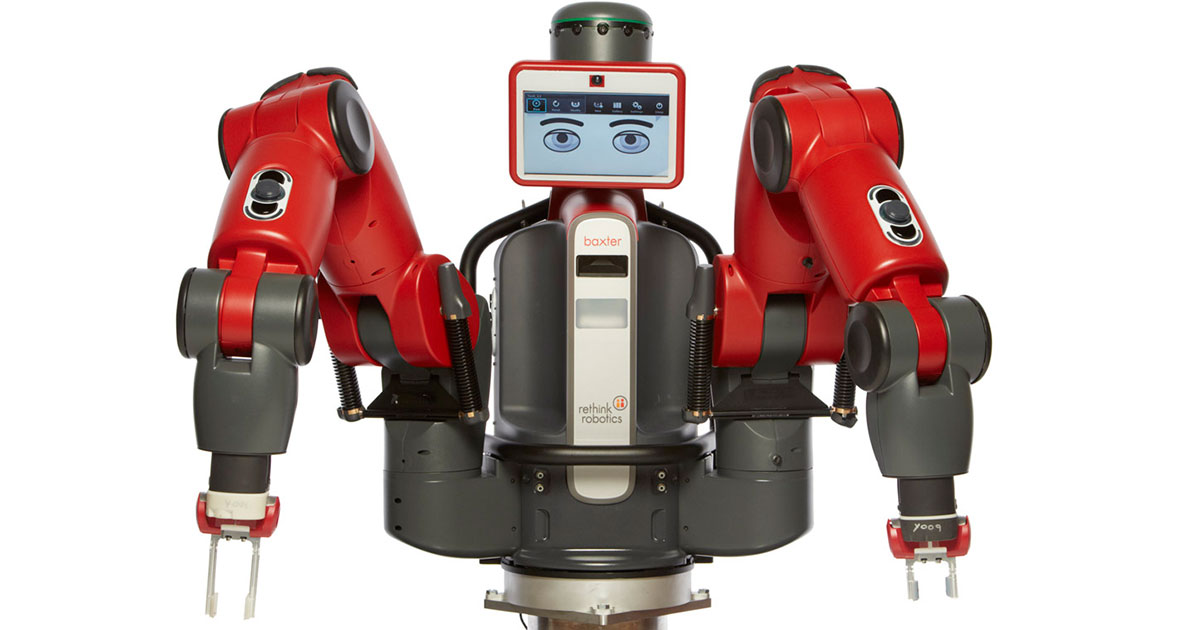
\includegraphics[height=0.45\textwidth]{inc/img/baxter}
  \caption{Антропоморфный робот \textit{Baxter}}
  \label{fig:baxter}
\end{figure}

Как отмечалось ранее, использование двух и более манипуляционных роботов в составе антропоморфного робота(рисунок \ref{fig:baxter}) позволяет совершать более сложные операции над объектом манипулирования. Кроме того, существует несколько других факторов, мотивирующих к использованию кооперации манипуляционных роботов:
\begin{itemize}
  \item \textbf{Сходство с человеком:} большое колличество коллаборативных роботов, в особенности домашние помощники и роботы, использующиеся в медицине, в частности в хирургии, адаптированы для взаимодействия с человеком и телеуправления посредством рук человека. Это дает возможность использовать эволюционно приобретенные человеческие навыки координации и манипулирования объектами в алгоритмах управления роботами \cite{coop_manipulator_survey};
  \item \textbf{Гибкость:}использование двух и более манипуляционных роботов позволяет получить большее колличество конфигураций благодаря увеличенному числу степеней подвижности. Это позволяет выполнять операции более энергоэфективно \cite{Ajoudani2017} или точно \cite{Faroni2016};
  \item \textbf{Грузоподъемность:} кооперация из манипуляторов может выполнять манипулирование объектами массой в разы большей, чем может поднять манипуляционный робот в одиночку \cite{AzizZadeh2019};
\end{itemize}

 Сейчас кооперативное управление можно разделить на два больших класса \cite{coop_manipulator_survey}: нескоординированное и скоординированное. Скоординированное управление можно также разделить на два типа: синхронизированное и бимануальное. Первое решает проблему планирования путей и траекторий для согласованного (без столкновений) движения нескольких манипуляторов. Второе же рассматривает несколько манипуляционных роботов как мультиагентную систему, каждый агент в которой принимает участие в выполнении одной общей для всех задачи. Кооперативная система манипуляционных роботов имеет большее число переменных состояния чем независимые роботы. Эти переменные состояния зачастую необходимы для управления, например контактное усилие, для удерживания предметов двумя роботами.

В связи с возросшим интересом к системам из двух и более манипуляционных роботов большую востребованность получили методы кооперативного управления манипуляторами, позволяющие выполнять такие задачи, как сборка деталей \cite{Sun2002}, механическая обработка деталей \cite{AzizZadeh2019}, удержание и позиционирование гибких и подвижных объектов \cite{Pfeffer1993} с заданными показателями качества управления. Разрабатываемый алгоритм кооперативного управления может быть использован в системах управления домашними роботами-помощниками, коллаборативными роботами, экзоскелетов, промышленных роботов, осуществляющих манипулирование тяжелыми объектами с высокой гибкостью реконфигурирования производства.

Для разработки алгоритма кооперативного управления в рамках данной работы ставятся следующие задачи:
\begin{enumerate}
  \item провести  обзор  литературных  источников,  рассматривающих  алгоритмы  гибридного позиционного/силомоментного  управления  для  одного  и  нескольких  артикулированных манипуляционных  роботов  за  последние  10  лет,  выделить  основные  методы,  описать  их достоинства   и   недостатки.   Обосновать   актуальность   рассматриваемой   задачи,
  \item рассмотреть   динамическую   и   кинематическую   модель   двух   артикулированных манипуляционных  роботов,  жестко  удерживающих  объект  в  заданных  точках  контакта. Масса и  вектор центра  масс объекта  считаются неизвестными.  Параметры  динамической модели  каждого  робота-манипулятора,  осуществляющего  манипулирование  объектом, считаются  известными.  Доступными  сигналами  для  управления  являются  моменты  на сочленениях каждого робота-манипулятора. Измеряемыми сигналами являются положение и  скорости  сочленений,  моменты  на  сочленениях,  а  также  силы  и  моменты  с датчиков, установленных   на   рабочем   инструменте   каждого   манипулятора,
  \item синтезировать   алгоритм   гибридного   силомоментного/позиционного   управления   для математической    модели    двух    артикулированных    манипуляционных    роботов, удерживающих объект, адаптивный к параметрической неопределенности модели объекта манипулирования,  обеспечивающий  статическую  ошибку  между  желаемыми  и  текущими положениями в рабочем пространстве не более 10 мм, силами и моментами действующимина  объект  манипулирования  не  более  20Н/50Нм  при  условии  наличия  полного  ранга матрицы  Якоби,  а  также  при  отсутствии  помех  измерений,  неучтенных  внешних  и параметрических  возмущений,
  \item провести  численное  моделирование  предложенного алгоритма  в  задаче  удерживании  заданного  постоянного  усилия  манипулируемым обьектом, с сохранением заданного положения.
\end{enumerate}






% Целью работы является создание всякой всячины. Для достижения поставленной цели необходимо решить следующие задачи:
%
% \begin{itemize}
% \item проанализировать существующую всячину;
% \item спроектировать свою, новую всячину;
% \item изготовить всякую всячину;
% \item проверить её работоспособность.
% \end{itemize}
%
% Проверяем как у нас работают сокращения, обозначения и определения "---
% MAX,
% \Abbrev{MAX}{Maximum ""--- максимальное значение параметра}
% API
% \Abbrev{API}{application programming interface ""--- внешний интерфейс взаимодействия с приложением}
% с обратным прокси.
% \Define{Обратный прокси}{тип прокси-сервера, который ретранслирует}
